\section{Results}
\label{sec:results}

In this section, we present the findings from our zero-shot classification and embedding analysis experiments.

\subsection{Zero-Shot Classification Performance}
\label{subsec:res_class}

Our evaluation of \gptmini reveals a moderate overall accuracy of \accuracy.
The model demonstrates highly non-uniform performance across the three modes, as detailed in \cref{tab:classification_results}.

\begin{table}[h]
\centering
\caption{Zero-shot classification results using \gptmini. The model perfectly identifies \aigen text but fails to detect \dictated text, which it misclassifies as either \aigen or \typed.}
\label{tab:classification_results}
\begin{tabular}{@{}lcccc@{}}
\toprule
\textbf{Mode} & \textbf{Precision} & \textbf{Recall} & \textbf{F1-Score} & \textbf{Support} \\
\midrule
\aigen & 0.65 & {\bf 1.00} & 0.79 & 50 \\
\dictated & 0.00 & 0.00 & 0.00 & 50 \\
\typed & 0.65 & 0.90 & 0.76 & 50 \\
\midrule
\textbf{Overall Accuracy} & \multicolumn{4}{c}{\bf \accuracy} \\
\bottomrule
\end{tabular}
\end{table}

{\bf Key Observations.}
\begin{itemize}[leftmargin=*]
    \item \aigen Detection: The model achieved 100\% recall for \aigen text, indicating that LLM-generated signatures are highly salient in zero-shot contexts.
    \item \dictated Failure: The model completely failed to identify the \dictated mode (0\% F1-Score). All 50 samples were misclassified as either \aigen (26 samples) or \typed (24 samples).
    \item \typed Precision: The model identified \typed text with 90\% recall and 65\% precision, suggesting that orthographic typos are recognizable but frequently confused with other modes.
\end{itemize}

\subsection{Embedding Cluster Analysis}
\label{subsec:res_embed}

Our analysis of the \minilm embedding space confirms that 'mode' acts as a latent variable with moderate separation.

{\bf Clustering Metrics.}
The Silhouette Score for the three mode-based clusters was \silhouette.
While not indicating perfect separation, this score reflects a significant degree of inherent structure in the embedding space that correlates with text origin.

{\bf PCA Results.}
The first principal component (PC1) explains \pcaone of the total variance, while the second (PC2) explains 5.1\%.
Visualization of these components (see \cref{fig:embedding_clusters}) shows a clear boundary separating \aigen text from the error-injected human modes (\dictated and \typed).
However, the regions corresponding to \dictated and \typed modes exhibit significant overlap along the primary latent axes, mirroring the confusion observed in the zero-shot classification experiment.

\begin{figure}[h]
\centering
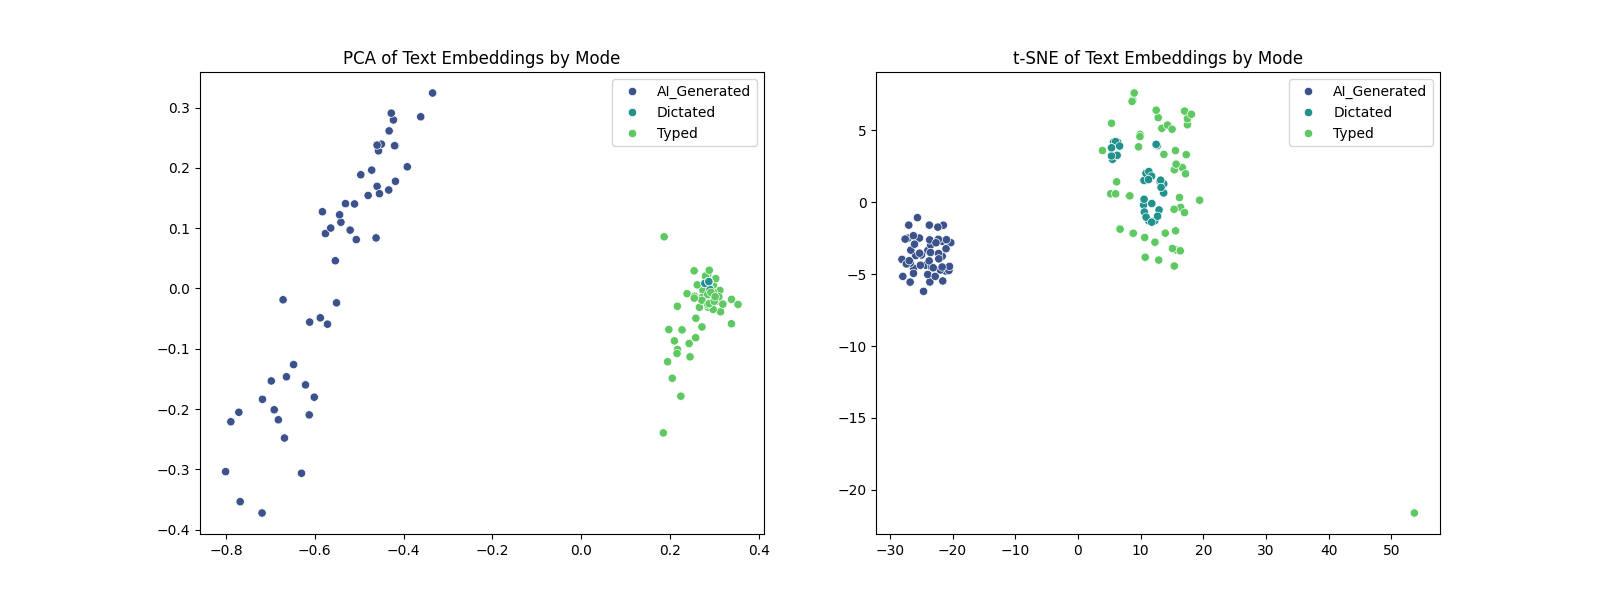
\includegraphics[width=0.8\linewidth]{figures/embedding_clusters.png}
\caption{Visualization of text embeddings using PCA. The first principal component (\pcaone variance) clearly separates \aigen samples (clusters on the left) from artifact-injected human text. However, \dictated and \typed modes show substantial overlap in the latent space.}
\label{fig:embedding_clusters}
\end{figure}
